\section{Use Case Diagram}
\label{sec:use_case_diagram}
% Begin Section
\begin{itemize}
	\item Provide the use case diagram for the system being developed.
	\item You do not need to provide the textual description of any of the use cases here (these will be specified under "Highlights of Functional Requirements").
	%	\item Provide \emph{one} use case diagram for the most important Business Event.
	%	\item The text of all use cases will be specified under "Highlights of Functional Requirements"
\end{itemize}


\begin{figure}
	% \includegraphics[width=\linewidth]{Example_Use_Case.png}
	\includegraphics[width=\linewidth]{Section3/Example_Use_Case.png}
	\caption{Use Case Diagram}
	\label{UseCaseDiagram}
\end{figure}
%In this section, select the most important Business Event that your system responds to and give its use case diagram.  Only one use case diagram is needed.  Give a brief textual description of the use case without repeating what is in the scenarios of the corresponding Business Event.

%
%
%
%This section should provide a use case diagram for your application. 
%\begin{enumerate}[a)]
%	\item Each use case appearing in the diagram should be accompanied by a text description. 
%\end{enumerate}
%% End Section